\documentclass[a4paper]{article}
\usepackage[utf8]{inputenc}
\usepackage{graphicx}
\usepackage{tabto}
\usepackage[
  left=3cm,
  right=2cm,
  top=2.5cm,
  bottom=2cm
]{geometry}

\title{Zusammenfassung Datenbanken}
\author{Heosibel}

\begin{document}

\maketitle


\begin{center}
    Sommersemester 2021 \\
    Professor: Dr.-Ing. Maik Thiele
\end{center}

\,

\begin{center}
    Dieses Dokument enthält eine Zusammenfassung der Vorlesung Datenbanken vom SS 2021.
    Diese Dokument ist kein offizielles vom Lehrstuhl und sollte nicht als Referenz verwendet werden.
    Die Erstellung ist in Vorbereitung auf die Prüfung im SS 2021 aus den Folien geschehen und kann Ungenauigkeit und/oder Fehler enthalten!
\end{center}


\newpage

\tableofcontents

\newpage

\section{Einführung}

\subsection{Definition Datenbank}
\begin{itemize}
    \item logisch konsistent  
    \item besitzt eine bestimmte Bedeutung
    \item repräsentiert einen Ausschnitt der realen Welt
\end{itemize}

\subsection{Ziel einer Datenbank}
\begin{itemize}
    \item effektives + effizientes Speichern
    \item Wiederfinden von Daten
    \item Analyse von Daten
\end{itemize}

\subsection{Gründe für DBS}
\begin{itemize}
    \item Effizienz und Skalierbarkeit
    \item Fehlerbehandlung und Toleranz
    \item Mehrbenutzersynchronisation
    \item Sicherstellung der Datenintegrität
    \item Deklarative Anfragesprachen ( Benutzer sagt was und nicht wie die Daten geholt werden)
    \item Datenunabhängigkeit
\end{itemize}

\subsection{ANSI-SPARC-Architektur}
\begin{itemize}
    \item Externe: Definition externer Schemata (Nutzer oder anwendungsspezifische Sichten)
    \item Logische: definiert die logischen Datenstrukturen und deren Beziehungen
    \item Interne: Festlegung der Art und Weise der Speicherung
\end{itemize}

\begin{figure}[htp]
    \centering
    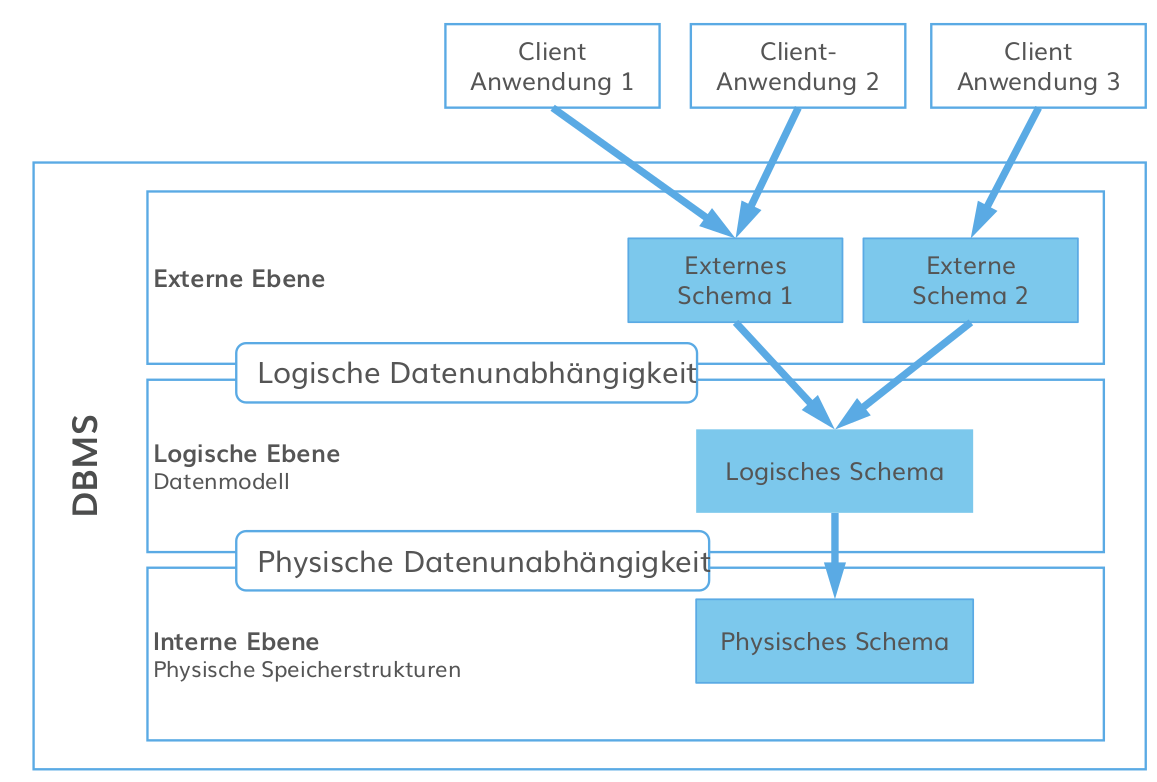
\includegraphics[width=9cm]{images/ANSI-SPARC}
    \caption{ANSI-SPARC-Architektur}
    \label{fig:ANSI-SPARC}
\end{figure}

\subsection{konzeptuelle Modelle}
\begin{itemize}
    \item Entity-Ralationship-Modell (ER-Modell)
    \item Unified Modeling Language (UML)
\end{itemize}

\subsection{Logische Modelle}
\begin{itemize}
    \item Hierarchische Modelle
    \item objektorientierte Modell
    \item Netzwerkmodelle
    \item Relationale Modelle
    \item ...
\end{itemize}

\subsection{Datenverwaltung ohne DBMS (Probleme)}
\begin{itemize}
    \item kein standardisiertes Format
    \item Duplikate
    \item hoher Aufwand bei Kombination von Daten
    \item Dateninkonsistenz
    \item maßgeschneidert aber ineffizient
    \item kein Mehrbenutzerzugriff
\end{itemize}

\newpage

\subsection{Information Retrieval}
\begin{itemize}
    \item Def: finden von Information unstrukturierter Art das eine Informationsnachfrage genügt
    \item Aufgabe:
    \begin{itemize}
        \item Suche nach Informationen
        \item Strukturierung von meist unstrukturierten Daten
        \item Befriedigung des Informationsbedürfnisses eines Benutzers
        \item Bewältigung von großen Datenmengen
    \end{itemize}
\end{itemize}

\subsection{Arten von Daten}
\begin{itemize}
    \item strukturierte Daten (z.B. Relationen)
    \item unstrukturiert Daten 
    \item semistrukturierte Daten
\end{itemize}


\section{Konzeptueller Entwurf}

\subsection{Phasen des Entwurfes}
\subsubsection{Konzeptueller Entwurf}
\begin{itemize}
    \item semantisches Modell der Objekttypen
    \item Beziehungen der Objekttypen
\end{itemize}

\subsubsection{Logischer Entwurf}
\begin{itemize}
    \item Transformation semantischen Modells in DBS-spezifisches Datenmodell
    \item z.B. ER-Modell
\end{itemize}

\subsubsection{Physischer Entwurf}
\begin{itemize}
    \item Einrichten der Datenbank + internes Schemata
    \item eventuell laden von Daten
\end{itemize}

\subsection{Entity-Relationship-Modell}
\begin{itemize}
    \item Entität: existiert in der Welt und unterscheidet sich von anderen Entitäten
    \item Attribut: relevantes Merkmal
    \item Beziehung: Zusammenhänge zwischen Entitäten
\end{itemize}


\subsection{Funktionalitäten}
\begin{itemize}
    \item One-To-One: (1:1) Beziehung von einer Entität zu höchstens einer anderen  
    \item Many-To-One: (1:N) 
    \item Many-To-Many: (N:M) Es liegt keine Beschränkung vor
    \item n-stellige Beziehungen (z.B. betreuen: Professoren x Studenten → Seminarthemen)
\end{itemize}

\subsection{Min/Max Notation}
\begin{itemize}
    \item min: jede Entität dieses Typs steht mind. min-mal in Beziehung
    \item max: jede Entität dieses Typs steht höchstens max-mal in Beziehung
    \item Sonderfälle
    \begin{itemize}
        \item min = 0: braucht keine Beziehungen
        \item max = *: kann beliebig oft in Beziehung stehen
    \end{itemize}
\end{itemize}

\begin{figure}[htp]
    \centering
    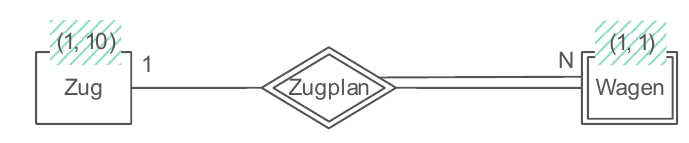
\includegraphics[width=9cm]{images/MinMaxNotation.png}
    \caption{Min-Max-Notation Beispiel Zug}
    \label{fig:MinMaxNotation}
\end{figure}

\subsection{erweiterte Attribut-Typen}
\begin{itemize}
    \item zusammengesetzte Datentypen
    \item mehrwertige Datentypen
    \item abgeleitet Attributwerte
\end{itemize}

\subsection{Spezialisierung und Generalisierung}
\begin{itemize}
    \item jede Instanz der Subklasse ist auch Instanz der Klasse
\end{itemize}
\begin{tabular}{l p{10cm}}
    Generalisierung (bottom-up): &  Unterdrückung der Unterschiede der Objekte \\
    & \\
    Spezialisierung (top-down): & Betonung der Unterschiede \\
    & \\
    d (disjunkt): & Instanzen der Unterklasse disjunkt \\
    & \\
    o (overlap): & Instanzen können sich überlappen \\
    & \\
    totale Spezialisierung: & Jede Instanz der Superklasse muss mind. eine Instanz der Subklasse sein \\
    & \\
    partielle Spezialisierung: & eine Instanz kann zu einer Subklasse gehören \\
    & \\
\end{tabular}

\begin{figure}[htp]
    \centering
    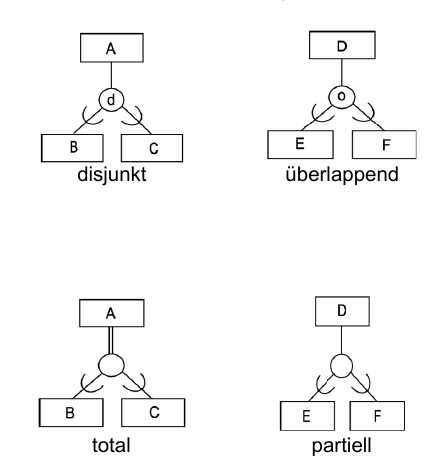
\includegraphics[width=4cm]{images/SpezialisierungGeneralisierung.png}
    \caption{Spezialisierung und Generalisierung Symbole}
    \label{fig:SpezialisierungGeneralisierung}
\end{figure}

\section{Logischer Entwurf}

\subsection{Grundlagen}
\begin{tabular}{l p{10cm}}
    Tupel: &  Element einer Relation \\
    & \\
    Kardinalität: & Kardinalität einer Relation: Anzahl der Tupel in einer Relation \\
    & \\
    Relation & Menge von Tupeln \\
\end{tabular}

\subsection{Primärschlüssel}
\begin{tabular}{l p{10cm}}
    Eindeutigkeit: &  jeder Schlüsselwert ist einzigartig und nicht doppelt vertreten \\
    & \\
    Definiertheit: & Jedes Objekt hat einen Schlüsselwert \\
    & \\
    Minimalität & es kann kein Teil des Schlüssels weggelassen werden sodass immer noch die Eigenschaften \\
\end{tabular}

\subsection{Fremdschlüssel}
\begin{tabular}{l p{10cm}}
    Verwendung: &  Ausdrücken von Beziehungen (verweist auf eine andere Relation wo dieser ein Primärschlüssel ist) \\
    & \\
    Eigenschaften: & Definiertheit und Minimalität
\end{tabular}

\subsection{ER-Modell in Relationales Modell}
\begin{enumerate}
    \item Übersetzung von Entitäten
    \item Übersetzung von Attributen
    \item Übersetzung von 1:1 Beziehungen
    \item Übersetzung von 1:N Beziehungen
    \item Übersetzung von M:N Beziehungen
    \item Übersetzung von Beziehungen zwischen mehr als zwei Relationen
    \item Übersetzung rekursiver Beziehungen
    \item Übersetzung von Attributen an Beziehungen
    \item Übersetzung von Vererbungsbeziehungen
\end{enumerate}

\subsection{Abbildungsvarianten}
\subsubsection{Horizontale Partitionierung}
\begin{itemize}
    \item jedes Objekt ist genau ein Tupel einer Relation → gleiche ID heißt nicht das selbe Objekt
    \item Zusammenführung der Gesamtrelation entstehen viele NULL Objekte
\end{itemize}

\subsubsection{Vertikale Zerlegung}
\begin{itemize}
    \item Gesamtheit aller Attribute einer Objektes nur durch den Verbund erhaltbar
\end{itemize}

\begin{figure}[htp]
    \centering
    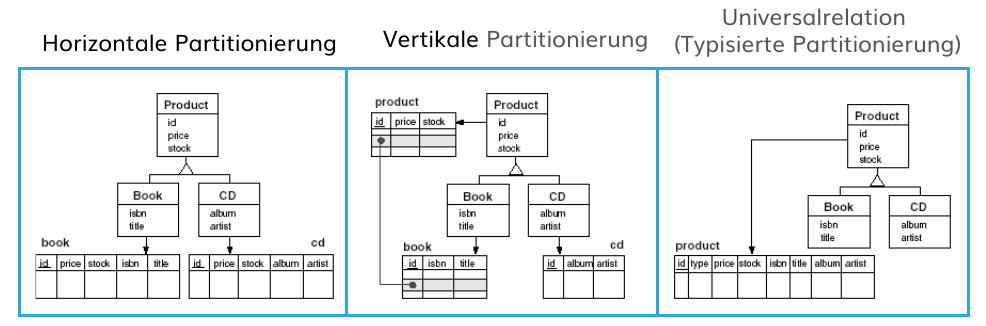
\includegraphics[width=14cm]{images/Partitionierung.png}
    \caption{Vertikale und Horizontale Partitionierung}
    \label{fig:Partitionierung}
\end{figure}

\newpage

\section{Relationale Algebra}
\begin{itemize}
    \item Formale Sprache von Anfrageergebnissen
    \item Nutzen zur Abfrageoptimierung
    \item enthält keine Operationen wie z.B. zum Erzeugen oder Löschen
\end{itemize}

\subsection{Basisoperationen}
\begin{tabular}{l p{11cm}}
    Projektion &  - Auswahl von bestimmten Spalten → erzeugen die neue Relational \\
     & - es dürfen keine Duplikate in der Projektion vorhanden sein (zu SQL verschieden) \\
     & \\
    Selektion & - ist die Menge aller Tupel die der Selektionsbedingung genügen \\
     & - Entspricht dem: SELECT * WHERE … \\
     & \\
    Kartesisches Produkt & Verknüpfung von allen Tupel der ersten Relation mit der zweiten\\
    & \\
    Vereinigung & entspricht der mathematischen Vereinigung von Mengen\\
    & \\
    Differenz & entspricht der mathematischen Differenz von Mengen
\end{tabular}

\subsection{Abgeleitete Operationen}
\begin{tabular}{p{3.5cm} p{11cm}}
    Durchschnitt & entspricht R-(R-S) \\
    & \\
    Division & \begin{itemize}
        \item Bei der Division von R $\div$ S bleiben die Attribute übrig, welche in jeder Kombination mit den Attributen aus S in R vorkommen
        \item $R \div S := \pi_{A-B}(R) - \pi_{A-B} ((\pi_{A-B}(R) \times S) -R) $
        \item Beispielfrage: welche Eltern haben Kinder mit dem Namen Maria (4) und Sabine (2) (siehe \ref{fig:Division})
    \end{itemize}\\
    Natürlicher Verbund & Verbund aller Elemente bei denen die Einträge übereinstimmen in in der Spalte mit gleicher Bezeichnung \\
    & \\
    Theta-Join & \begin{itemize}
        \item Verbund von Relationen bezüglich beliebiger Attribute und einem Selektionsprädikat
        \item selbes Ergebnis, kann durch Bildung des kartesische Produkt und nachträglicher  Kontrolle der Bedingung erzielt werden
    \end{itemize}\\
    
    Equi-Join & \begin{itemize}
        \item entspricht dem INNER JOIN in SQL
        \item Bildung des kartesischen Produkt und Kontrolle bestimmter Spalten auf Äquivalenz
    \end{itemize}\\
    
    Left-Outer-Join & \begin{itemize}
        \item alle Tupel der linken Relation, die kein Join Partner in der rechten Relation haben werden dennoch ausgegeben
        \item entsprechende Spalten haben NULL Werte
    \end{itemize}\\
    
    Right-Outer-Join & alle Tupel der rechten Relation, die kein Join-Partner in der linken Relation haben werden dennoch ausgegeben \\
    & \\
    Full-Outer-Join & alle Tupel sowohl der linken als auch der rechten Relation die keinen Join Partner haben werden trotzdem ausgegeben \\
    & \\
    Halbverbund  & Für zwei Relationen R und S ist das Ergebnis des halben natürlichen Verbundes
\end{tabular}

\begin{figure} [htp]
    \centering
    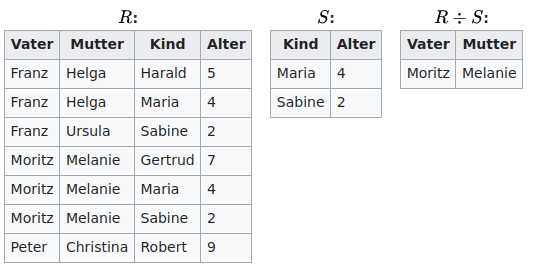
\includegraphics[width=8cm]{images/Division.png}
    \caption{Division Veranschaulichung}
    \label{fig:Division}
\end{figure}


\section{Entwurfstheorie}

\subsection{Anomalien}
\begin{tabular}{l l}
     Insert-Anomalie&  Vermischung zweier Entitätstypen\\
     & \\
     Update-Anomalie & Redundanz innerhalb der Relation \\
     & \\
     Delete-Anomalie & Verlieren der Verbindung zu einer Entität durch löschen einer anderen
\end{tabular}

\subsection{Entwurfsziele}
\begin{itemize}
    \item Vermeidung von Redundanzen und Anomalien
    \item Vermeidung von Informationsverlust
    \item Effizienzüberlegungen
\end{itemize}

\subsection{Normalisierung Übersicht}
\begin{itemize}
    \item Eliminierung von Redundanzen
    \item Vermeidung von Änderungsanomalien (Beseitigung von Abhängigkeiten) 
    \item 1. NF: keine mehrwertigen Attribute
    \item 2. NF: keine Vermischung von Sachverhalten
    \item 3. NF: keine funktionalen Abhängigkeiten von Nichtschlüsselattributen
\end{itemize}

\subsection{1. Normalform}
\begin{itemize}
    \item alle Attribute der Relation sind atomar (mehrwertige Attribute sind nicht erlaubt)
    \item Definition atomar hängt vom Sachverhalt ab
    \item Wertebereich ist STRING und INTEGER
\end{itemize}

\subsection{Funktionale Abhängigkeiten}
A und B sind Attributmengen, dann ist B von A funktional abhängig gdw. Für alle real möglichen Relationen r(RS) zu jedem Wert in A genau ein Wert in B gehört.

\vspace{5mm}

\begin{tabular}{l p{12cm}}
     voll funktional abhängig & alle Attribute in X sind für die funktional Abhängigkeit notwendig \\
     & \\
     partielle abhängig & es sind nicht alle Attribute notwendig\\
     & \\
     Superschlüssel & A ist ein Superschlüssel wenn dies alle anderen Attributwerte bestimmt, A muss nicht minimal sein (RS → SR gilt immer)\\
     & \\
     Kandidatenschlüssel & \begin{itemize}
         \item ist Vollständig und Minimal
         \item es kann mehr als einen in einer Relation geben
         \item bildet den Primärschlüssel einer Relation
     \end{itemize} \\
\end{tabular}

\begin{tabular}{l p{10cm}}
     
     Hülle von F & Eine Hülle F+, ist die Menge aller funktionalen Abhängigkeiten die aus den funktionalen Abhängigkeiten in F ableitbar sind \\
     & \\
     Armstrong Axiome & \begin{itemize}
         \item Vereinigungsregel: falls $A \rightarrow B$ und $A \rightarrow C$, dann gilt auch $A \rightarrow B \cup C$
         \item Dekompositionsregel: falls $A \rightarrow B \cup C$ ,dann gilt auch $A \rightarrow B$ und $A \rightarrow C$
         \item Pseudotransivität: falls $A \rightarrow B$ und $B \cup C \rightarrow D$, dann  auch $A \cup C \rightarrow D$
     \end{itemize}
\end{tabular}

\subsection{Zerlegung von Relationen}
\subsubsection{Verlustlosigkeit}
\begin{itemize}
    \item Die Ursprungsrelation R muss wieder aus den Teilrelationen hergestellt werden können (über joins)
    \item es liegt kein Informationsverlust vor wenn für die Teilrelationen RS1 und RS2 gilt:
    \begin{itemize}
        \item $(RS_1 \cap RS_2 \rightarrow RS_1) \in F^+$ oder 
        \item $(RS_1 \cap RS_2 \rightarrow RS_2) \in F^+$
    \end{itemize}
\end{itemize}

\subsubsection{Abhängigkeitserhaltung}
\begin{itemize}
    \item die funktionalen Abhängigkeiten müssen auf die Schemata RS1, RS2, … übertragbar sein
    \item es wird eine hüllentreue Zerlegung gefordert: $F_{RS}^+ = (F_{RS_1} \cup ... \cup F_{RS_n})^+$ 
\end{itemize}

\subsection{2. Normalform}
\begin{itemize}
    \item jedes Attribut ist entweder
    \begin{itemize}
        \item teil eines Kandidatenschlüssel oder
        \item von jedem Kandidatenschlüssel voll funktional abhängig
    \end{itemize}
    \item Verstoß gegen 2NF weißt auf Vermischung von verschieden Beziehungen 
\end{itemize}

\subsection{3. Normalform}
\begin{itemize}
    \item für alle Abhängigkeit $X \rightarrow A$ mit $X \subset R, A \in R, A \notin X$ gilt:
    \begin{itemize}
        \item X enthält einen Schlüssel von R oder
        \item A ist Teil eines Schlüsselkandidaten
    \end{itemize}
    \item 3NF beseitigt Abhängigkeiten von Nicht-Schlüsselattributen
\end{itemize}

\subsection{Kanonische Überdeckung}
\begin{enumerate}
    \item Schritt: Linksreduktion
    \begin{itemize}
        \item für alle $A \rightarrow B$ in F überprüfe ob durch weglassen von einem Element auf der linken Seite auch B anderes erreicht werden kann
        \item Nur Betrachtung von Abbildungen mit mind. 2 Elementen auf der linken Seite
        \item z.B.: $AB \rightarrow C, A \rightarrow E, E \rightarrow B$, es kann B weggelassen werden da B in der Hülle(F,A) = {A,B,C,E} ist 
    \end{itemize}
    
    \item Schritt: Rechtsreduktion
    \begin{itemize}
        \item ein Element auf der rechten Seite kann weggelassen werden und ist dennoch über andere Wege erreichbar
        \item z.B.: $A \rightarrow BC, E \rightarrow BF, A \rightarrow DE$, B kann weggelassen werden da $A \rightarrow E \rightarrow B$ abbildet
    \end{itemize}
    \item Schritt: Entfernen von FD‘s mit leerer Menge auf der rechten Seite
    \item Schritt: Zusammenfassung von FD mit gleicher linken Seite
\end{enumerate}

\subsection{3NF-Synthesealgorithmus}
\begin{itemize}
    \item Zerlegung eines Relationsschemas R mit funktionalen Abhängigkeiten in Relationsschemata $R_1, ... ,R_n$ es muss erfüllt sein:
    \begin{itemize}
        \item kein Informationsverlust
        \item Bewahrung der funktionalen Abhängigkeiten
        \item $R_1 , ... ,R_n $ erfüllen dritte Normalform
    \end{itemize}
    \item Generierung der Zerlegung
    \begin{enumerate}
        \item bestimme die kanonische Überdeckung $F_c$ der Menge F
        \item für alle FD in $F_c$ erstelle eine Relation (z.B. $A \to BC$ erzeugt $R_A$ = {A,B,C})
        \item falls kein Schlüsselkandidat der Ursprungsrelation enthalten erzeuge einen zusätzlichen $R_K$ = K wobei K ein Schlüsselkandidat von R ist
        \item Entferne doppelte Schemata (z.B. $R_1:{A,B,C,D}$ ; $R_2:{A,C} \Rightarrow R2$ ist schon in $R_1$)
    \end{enumerate}
\end{itemize}

\subsection{Boyce-Codd-Normalform}
\begin{itemize}
    \item für alle Abhängigkeiten $X \to A$ gilt: X enthält einen Schlüssel von R
    \item beseitigt Abhängigkeiten unter Attributen, die Teil eines Schlüsselkandidaten sind
    \item Herstellung von BCNF
    \begin{itemize}
        \item Zerlegung von R in R1 und R2
        \item Erstelle eine List der Determinanten
        \item für jede Determinante die kein Schlüsselkandidat ist erstelle eine neue Relation
        \item Erhalte nur die Determinante in der Originalrelation
    \end{itemize}
\end{itemize}


\section{Transaktionsverwaltung}
\begin{itemize}
    \item Teilgebiete
    \begin{itemize}
        \item Synchronisation von mehreren gleichzeitig ablaufenden Transaktionen
        \item Recovery von eingetretenen, oft unvermeidbaren Fehlersituationen
    \end{itemize}
    \item Transaktion: Zusammenfassung von aufeinanderfolgenden DB-Operationen
\end{itemize}

\subsection{Operationen}
\begin{tabular}{l l}
    BOT & Begin of transaction \\
    & \\
     Commit & Erfolgreiches Beenden einer Transaktion \\
     & \\
     Abort & Selbstabbruch der Transaktion $\to$ Zurücksetzen der Datenbasis \\
     & \\
     define savepoint & fest definierter Sicherungspunkt \\
     & \\
     backup transaction & zurücksetzen der aktiven Transaktion auf einen Sicherungspunkt \\
\end{tabular}

\subsection{ACID-Eigenschaften}
\begin{tabular}{l p{12cm}}
     Atomarität &  Transaktionen beginnen mit einem BOT und enden mit EOT (Alles oder nichts Prinzip)\\
     & \\
     Konsistenzerhaltung & einer erfolgreiche Transaktion garantiert die Konsistenzbedingungen \\
     & \\
     Isolation & unterschiedliche Transaktionen laufen isoliert voneinander ab \\
     & \\
     Dauerhaftigkeit & Ergebnisse erfolgreicher Transaktionen müssen persistent sein
\end{tabular}

\subsection{Anomalien ohne Synchronisation}
\begin{itemize}
    \item Verlorengegangene Änderungen (lost update)
    \item Abhängigkeiten von nicht freigegeben Änderungen (dirty read, dirty overwrite)
    \item Inkonsistente Analyse (non repeatable read)
    \item Phantom-Problem
\end{itemize}

\subsection{ANSI-SQL Isolationsstufen}
\begin{figure} [htp]
    \centering
    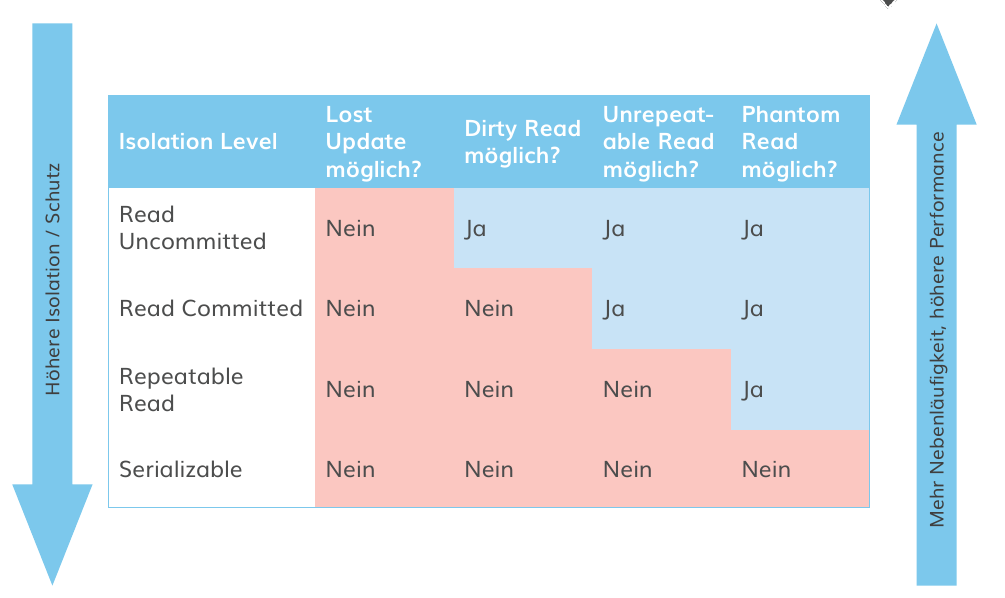
\includegraphics[width=10cm]{images/ANSI-Isolationsstufen.png}
    \caption{ANSI-SQL Isolationsstufen}
    \label{fig:Isolationsstufen}
\end{figure}

\subsection{Serialisierbarkeitstheorie}
\begin{itemize}
    \item Operationen einer Transaktionen
    \begin{itemize}
        \item Leseoperation $r_j(A)$
        \item Schreiboperation: $w_j(A)$
        \item Abbruch $a_j$
        \item Commit $c_j$
    \end{itemize}
    \item Ausführungsplan: nebenläufiges Ausführung von mehrere TA
    \item Konfliktoperationen
    \begin{itemize}
        \item zwei Operationen arbeiten auf dem selben Datenobjekt
        \item eine ist mind. eine Schreiboperation
    \end{itemize}
    
    \item Serialisierbarkeit
    \begin{itemize}
        \item sequenzielle Ausführung führt zu lange Wartezeiten und schlechter Auslastung
        \item serialisierbarer Ablaufplan durch
        \begin{itemize}
            \item Beschränkung der ''Parallelität'' auf erlaubte Verarbeitungsreihenfolgen
            \item Äquivalenz zu einer seriellen Historie
            \item serialisierbare Ablaufpläne sind korrekt und frei von Anomalien
        \end{itemize}
        \item Achtung: zwei Ablaufpläne können zu unterschiedlichen Ergebnissen führen
    \end{itemize}
        
    \item Serialisierbarkeitsgraph
    \begin{itemize}
        \item Ablaufplan ist serialisierbar, wenn der Serialisierbarkeitsgraph keine Zyklen enthält
        \item Serialisierbarkeitsgraph
        \begin{itemize}
            \item Knoten: einzelne Transaktion
            \item Kanten: Abhängigkeiten zwischen 2 Transaktionen
        \end{itemize}
    \end{itemize}
\end{itemize}

\subsection{weitere Eigenschaften von Transaktionen}
\begin{itemize}
    \item Rücksetzbarkeit
    
    \begin{itemize}
        \item abgeschlossene Transaktionen dürfen nicht zurückgesetzt werden
        \item Abschluss einer TA nur wenn alle TA von denen sie gelesen hat abgeschlossen sind
        \item Mindestvoraussetzung für die Dauerhaftigkeit
        \item commit Reihenfolge muss eingehalten werden
    \end{itemize}
    
    \item Vermeidung kaskadierenden Rücksetzens
    
    \begin{itemize}
        \item TA dürfen nur Ergebnisse von abgeschlossen TA sehen
    \end{itemize}
    
    \item Striktheit
    
    \begin{itemize}
        \item Rücksetzen durch ein Befor-Image
        \item veränderte Objekte dürfen nicht verändert werden bevor die aktuelle TA abgeschlossen ist
    \end{itemize}
    
\end{itemize}

\subsection{Datenbank-Scheduler}
\begin{itemize}
    \item ordnet eingehende Operationen und sorgt für serialisierbare und rücksetzbare Historien
\end{itemize}

    \subsubsection{Pessimistischer Scheduler}
    \begin{itemize}
        \item verzögert entgegengenommene Operationen
        \item bei mehreren Operationen Festlegung einer geschickten Reihenfolge
    \end{itemize}

    \subsubsection{Optimistischer Scheduler}
    \begin{itemize}
        \item schnelle Auführung neuer eingehender Operationen 
        \item eventuell später Schaden reparieren
    \end{itemize}

\subsection{Synchronisation durch Sperren (Pessimistische Synchronisation)}

    \subsubsection{Pessimistische Synchronisation}
    \begin{itemize}
        \item Sperren für exklusiven Zugriff auf Datenobjekte
        \item zentrale Sperrtabelle für die Nutzungsart
        \item Arten von Sperren
        
        \begin{itemize}
            \item X (eXkclusive)-Sprre (=Schreibsperre)
            \item S/R (shared/read)-Sperre (=Lesesperre)
        \end{itemize}
    \end{itemize}
    
    \subsubsection{Statisches Sperren}
    \begin{itemize}
        \item zum Beginn der TA Anforderung aller Sperren
        \item Nachteil: Sperren von allem was man brauchen könnte
    \end{itemize}

    \subsubsection{Dynamisches Sperren}
    \begin{itemize}
        \item Anforderung von Sperren nach Bedarf
        \item Nachteil: Verklemmungen (Deadlocks)
    \end{itemize}

    \subsubsection{Zweiphasen-Sperrprotokoll}
    \begin{itemize}
        \item Wachstumsphase: Sperren werden angefordert aber keine freigegeben
        \item Schumpfungsphase: Sperren freigegeben aber keine angefordert
    \end{itemize}

    \subsubsection{Striktes Zweiphase-Sperrprotokoll}
    \begin{itemize}
        \item Freigabe aller Schreibsperren erst am  Ende einer Transaktion
        \item Freigabe Lesesperre entsprechend Standard-2PL-Verfahren
        \item Vorteil: verhindert kaskadierendes Zurücksetzen
        \item Nachteil: Sperren werden zu lange gehalten
    \end{itemize}
    

\subsection{Deadlocks}
\begin{itemize}
    \item Verklemmungen können bei pessimistischen Methoden nicht verhindert werden
    \item Deadlock: Abhängigkeit von TA die wechselseitig auf Freigabe von Sperren warten
\end{itemize}

    \subsubsection{Deadlockerkennung}
    \begin{itemize}
        \item Erzeugung eines Wartegraphen der TA
        \item prüfen auf Zyklen im Graphen → bei Zyklus eine TA zurücksetzen
        \item Kriterien für Zurücksetzen: Alter, Fortschritt, Anzahl Sperren, Abhängige TA, …
    \end{itemize}

    \subsubsection{Deadlockvermeidung}
    \begin{itemize}
        \item versucht eine TA eine Sperre zu erwerben die vergeben ist setzt sich eine TA zurück
        \item Vermeidungsstrategien: Wait-Die und Wound-Wait
        \item Wait-Die
        
        \begin{itemize}
            \item Fordert T1 eine Sperre an die von einer jüngeren T2 gehalten wird wartet T1 bis die Sperre freigegeben wird
            \item Fordert T1 eine Sperre an die von einer älteren T2 gehalten wird, startet T1 mit dem alten Zeitstempel neu
        \end{itemize}
        
        \item Wound-wait
        \begin{itemize}
            \item Fordert T1 eine Sperre an die von einer jüngeren T2 gehalten wird, startet T2 neu und sie Sperre wird an T1 übergeben
            \item Fordert T1 eine Sperre an die von einer älteren T2 gehalten wird, so wartet T1 bis die Sperre von T2 freigegeben wird
        \end{itemize}
    \end{itemize}

\subsection{Optimistische Synchronisation}
\begin{itemize}
    \item Forderung: TA kann validieren, wenn alle zuvor validierten TA gesehen wurden
\end{itemize}

    \subsubsection{3 phasige Verarbeitung}
    \begin{itemize}
        \item Lesephase
        
        \begin{itemize}
            \item eigentliche TA-Verarbeitung
            \item Änderungen werden im den privaten Puffer durchgeführt
        \end{itemize}
        
        \item Validierungsphase
        
        \begin{itemize}
            \item Überprüfung auf Konflikte mit parallel abgelaufenen TA
            \item Konfliktlösung durch Zurücksetzen
        \end{itemize}
        
        \item Schreibphase
        
        \begin{itemize}
            \item nur bei positiver Validierung
            \item Lese-TA ohne Zusatzaufwand
            \item Schreib-TA schreiben LOG-Information und propagieren Änderungen
        \end{itemize}
    \end{itemize}
    
    \subsubsection{Backward Oriented}
    \begin{itemize}
        \item Validierung gegenüber bereits beendete TA
        \item Nachteile:
        
        \begin{itemize}
            \item Aufbewahrung der Write-Sets beendeter Transaktionen nötig
            \item hohe Anzahl an Vergleichen bei Validierung
        \end{itemize}
        
    \end{itemize}
    
    \subsubsection{Forward Oriented}
    \begin{itemize}
        \item Validierung gegenüber laufenden TA
        \item Vorteil: Frühzeitiges Rücksetzen möglich → Einsparung von Arbeit
        \item Probleme: hohe Rücksetzraten möglich
    \end{itemize}

\subsection{Recovery}
\begin{itemize}
    \item Alles oder Nichts Prinzip von TA
    \item Voraussetzung: Sammlung redundanter Informationen während des Betriebes
    \item Sicherungspunkte: Schnappschuss des Datenbankinhaltes
    \item Log-Datei: Protokollierung aller Änderungen in einer Datei
\end{itemize}
    
    \subsubsection{Fehlerarten}
    \begin{tabular}{l l }
        Transaktionsfehler: &  Anwendungsbedingter Fehler (falsche Operation/Wert)\\
        & \\
        Systemfehler: & Systemzusammenbruch mit Verlust des Hauptspeichers \\
        & \\
        Gerätefehler: & Zerstörung Sekundärspeicher \\
        & \\
        Katastrophen: & Zerstörung des Rechenzentrums
    \end{tabular}
    
    \subsubsection{Recorvery-Klassen}
    \begin{tabular}{l p{7.5cm}}
        Lokaler Fehler: &  Fehler in einer nicht abgeschlossen TA $\to$ lokales undo (R1)\\
        Fehler mit Hauptspeicherverlust: & abgeschlossen bleiben erhalten, andere werden zurückgesetzt \\
        Fehler mit Hintergrundspeicherverlust: & Behebung mittels Archivkopie+Logarchiv (R4)
    \end{tabular}
    
    \subsubsection{Ersetzungsstrategien}
    \begin{itemize}
        \item STEAL
        
        \begin{itemize}
            \item geänderte Seiten können vor EOT in den Hintergrundspeicher verdrängt werden
            \item Speicherung von Undo-Informationen nötig (Write-Ahead-Log Prinzip)
        \end{itemize}
        
        \item NOSTEAL : Seiten mit schmutzigen Änderungen dürfen nicht ersetzt werden
    
        
        \item FORCE
        
        \begin{itemize}
            \item geänderte Seiten werden spätestens bei EOT persistent gespeichert
            \item hoher Schreibaufwand, DB Puffer werden schlecht genutzt
        \end{itemize}
        
        \item NOFORCE
        
        \begin{itemize}
            \item geänderte Seiten können später erst persistent gespeichert werden
            \item Einhaltung der Commit Regel
            \item Redo-Recovery nach Rechnerausfall
        \end{itemize}
    \end{itemize}

    \subsubsection{Einbringstrategien}
    \begin{tabular}{l p{11cm}}
         Update in Place: & jede Seite hat genau eine Heimat, wo der alte Zustand überschrieben wird \\
         Twin-Block-Verfahren: & jede Seite hat 2 Seiten im Hintergrundspeicher, die vorletzte wird immer überschrieben\\
         Schattenspeicherkonzept: & nur geänderte Seiten werden dupliziert
    \end{tabular}
    
    \subsubsection{Protokollierungsarten}
    \begin{itemize}
        \item Logische Protokollierung
        
        \begin{itemize}
            \item Undo-Operation → vorherigen Zustand zu erzeugen
            \item Redo-Operation → Nachfolgerzustand zu erzeugen
        \end{itemize}
        
        \item Physische Protokollierung
        
        \begin{itemize}
            \item before-Image des Datenobjektes → statt Undo-Operation
            \item fter-Image des Datenobjektes → statt Redo-Operation
        \end{itemize}
        
        \item Redo-Informationen: Wiederholung von Änderung möglich
        \item Undo-Informationen: rückgängig machen von Änderungen 
    \end{itemize}

    \subsubsection{Zusätzliche Log Komponenten}
    \begin{tabular}{l l}
         LSN: &  Log Sequenz Number - Eindeutige Kennungsnummer\\
         Transaktionserkennung & \\
         PageID: & Seitenkennung der Änderung\\
         PrevLSN: & Zeiger auf vorherigen Log Eintrag
    \end{tabular}
    
    \subsubsection{Wiederanlauf nach einem Fehler}
    \begin{enumerate}
        \item Analyse: Ermittlung Winner (abgelossene TA) /Looser TA
        \item Redo: erneute Ausführung aller Änderungen (Winner und Looser), Vergleich mit LSN
        \item Undo: rückgängige Ausführung der Looser TA(Compensations Log Records)
    \end{enumerate}

\subsection{Sicherungspunkte}
\begin{itemize}
    \item Begrenzung des Redo-Aufwandes nach Systemfehler
    \item kritisch: Hot-Spot-Seiten ( Seiten die fast nie verdrängt werden)
\end{itemize}

    \subsubsection{Sicherungspunktarten}
    \begin{itemize}
        \item transaktionskonsistente Sicherungspunkte
        
        \begin{itemize}
            \item DBS Überführung in ein Ruhezustand → aktive TA beenden, neue verschieben
            \item sehr aufwendig, nur im Ausnahmefall möglich
        \end{itemize}
        
        \item aktionskonsistente Sicherungspunkte
        
        \begin{itemize}
            \item Abschluss aller elementaren Änderungsoperationen
            \item Übertragung aller modifizierten Seiten in den Hintergrundspeicher
            \item Redo-Informationen können gelöscht werden bis zum Sicherungspunkt, Undo nicht
        \end{itemize}
        
        \item unscharfe (fuzzy) Sicherungspunkte
        
        \begin{itemize}
            \item modifizierte Seiten werden nicht ausgeschrieben nur deren Kennung
            \item Dirty-Pages = Menge modifizierter Seiten
            \item MinDirtyPagesLSN: min LSN deren Änderung noch nicht ausgeschrieben wurde
        \end{itemize}
    \end{itemize}

\section{Indexstrukturen}

\subsection{Zugriffsarten}
\begin{itemize}
    \item sequenzieller Zugriff auf alle Sätze
    \item sequenzieller Zugriff in Sortierreihenfolge
    \item direkter Zugriff auf Primärschlüssel
    \item direkter Zugriff auf Sekundärschlüssel
    \item direkter Zugriff auf zusammengesetzte Schlüssel
    \item navigierender Zugriffe
\end{itemize}

\subsection{DB-Scan vs Index-Nutzung}

    \subsubsection{DB-Scan}
    \begin{itemize}
        \item alle Blöcke müssen gelesen und untersucht werden
        \item ausreichend bei Anfragen mit großer Treffermenge
        \item Optimierung durch Prefetching
    \end{itemize}
    
    \subsubsection{Index-Nutzung}
    \begin{itemize}
        \item Schlüsselwerte werden transformiert (Hash-Verfahren)
        \item Schlüsselwert werden redundant in eigener Struktur gehalten (z.B. Baum)
        \item wenn kann Zugriffspfad vorhanden $\to$ DB-Scan
    \end{itemize}

\subsection{Primär und Sekundärindex}
\begin{itemize}
    \item Primärindex: Dateiorganisationsformen
    
    \begin{itemize}
        \item unsortierte Speicherung von Tupel (Heap)
        \item sortierte Speicherung von internen Tupeln
        \item gestreute Speicherung von internen Tupeln
        \item Speicherung in mehrdimensionalen Räumen
        \item Normalfall: Primärindex über Primärschlüssel / geclusterter Index
    \end{itemize}
    
    \item Sekundärindex
    
    \begin{itemize}
        \item redundante Zugriffsmöglichkeiten, zusätzliche Zugriffspfade
    \end{itemize}
\end{itemize}

\subsection{B-Baum der Ordnung k}
\begin{itemize}
    \item jeder Knoten enthält höchstens 2k Schlüssel und mind k Schlüssel
    \item die Wurzel enthält mind einen Schlüssel $\to$ mind Speicherplatznutung $\ge$ 50\%
    \item Knoten mit k Schlüsseln hat k+1 Kinder
    \item alle Blätter sind auf dem selben Level
\end{itemize}

    \subsubsection{Einfügen eines neuen Schlüssels (stets ein Blatt)}
    \begin{itemize}
        \item Einfügen des neuen Schlüssel in der entsprechenden Stelle
        \item kann zu Überlauf führen (s = 2k +1) $\to$ splitten des Knoten
        \item Überläufe können sich bis zur Wurzel propagieren
    \end{itemize}
    
    \subsubsection{Entfernen eines Schlüssels}
    \begin{itemize}
        \item entweder löschen aus Blatt oder innerer Knoten → Rückführung auf ein Blatt
        \item Anzahl der Schlüssel nach Entfernen
        
        \begin{itemize}
            \item $s > k \to Stop$
            \item $s = k-1 \to$ Unterlauf
            
            \begin{itemize}
                \item Fall 1: Geschwisterknoten hat $\ge k+1$ Schlüssel $\to$ Ausgleich Geschwisterknoten
                \item Fall 2: Geschwisterknoten hat k Schlüssel $\to$ Verschmelzung mit Geschwister und Hinzunahme Vaterschlüssel
            \end{itemize}
        \end{itemize}
    \end{itemize}

\subsection{$B^+-Baum$}
\begin{itemize}
    \item jeder Pfad von Wurzel zu Blatt hat die gleiche Länge
    \item jeder Knoten (außer Wurzel) hat mind k und höchstens 2k Einträge
    \item alle Sätze werden in Blattknoten abgelegt
    \item innere Knoten enthalten nur die Verzweigungsinformation aber keine Daten
    \item jeder Blattknoten hat eine Referenz zu seinen beiden Nachbarn
\end{itemize}

    \subsubsection{Einfügen eines Eintrages}
    Wie im B – Baum nur das die Referenz nach oben geschoben werden ohne die Daten
    
    \subsubsection{Entfernen von Einträgen}
    \begin{itemize}
        \item Fall 1: $s > k \to$ Stop
        \item Fall 2: $s = k-1 \to$ Unterlauf: Mische Blatt mit Geschwisterknoten
        
        \begin{itemize}
            \item Fall 1: Summe Einträge $ \le 2k \to $ Zusammenfassung Blätter + Unterläufe behandeln
            \item Fall 2: Summe Einträge $ >  2k \to$ Teile Sätze neu auf beide Knoten auf (Hälfte) + aktualisiere Diskiminator im Vaterknoten
        \end{itemize}
    \end{itemize}

\subsection{Vergleich B-Baum und $B^+$-Baum}
\begin{tabular}{|c|c|}
    \hline
    \textbf{B-Baum}  & \textbf{$B^+$-Baum} \\
    \hline
    Keine Redundanz & Teilweise redundant \\
    \hline
    Einbettung der Datensätze $\to$ große Höhe & Blattknotenkette liefert Sortierte Schlüsselwerte \\
    \hline
    Wenige 1 Schritt Zugriffe in der Wurzel & Geringe Höhe durch hohe Verzweigung \\
    \hline
\end{tabular}
\begin{itemize}
    \item B-Bäume sinnvoll für Prädikate mit geringem Verhältnis zwischen Ein-und Ausgangskardinalität
    \item Daumenregel: Grenztrefferrate ca. 5\%
\end{itemize}

\subsection{Hashverfahren}
Ziele: 
\begin{itemize}
    \item direkter Zugriff nach Schlüsselwert
    \item Anzahl der Seitenzugriffe nahe 1 $\to$ Kollisionen unerwünscht
    \item effiziente Speichernutzung
\end{itemize}

    \subsubsection{Divisionsrestverfahren (Restklassenbildung)}
    \begin{itemize}
        \item Bitdarstellung der Zahlen
        \item $h(s) =$ s mod q (q größte Primzahl $ \le |N| \leftarrow $ liefert eine zulässige Adresse)
    \end{itemize}
    
    \subsubsection{Faltung}
    \begin{itemize}
        \item Zerlegung von k in einzelne Bestandteile
        \item Deren Verknüpfung additiv, multiplikativ oder logisch
        \item Ergebnis als Binärzahl interpretieren und dem Adressraum anpassen
    \end{itemize}
    
    \subsubsection{Techniken zur Kollisionsbehandlung}
    \begin{enumerate}
        \item Verkettung
        
        \begin{itemize}
            \item Seperates Verketten
            \begin{itemize}
                \item Verkettung der Elemente mit gleichem Hash-Wert/Bucketnummer
                \item Problem: Speicherung vieler Pointer
            \end{itemize}
            
            \item Überlaufbereiche
            \begin{itemize}
                \item Buckets fester Größe pro Hash-Wert
                \item Verkettung von Buckets → weniger Pointer
                \item Problem: Variierende Seitenzugriffe beim Suchen
            \end{itemize}
        \end{itemize}
        
        \item Open Addressing (Lineares Sondieren)
        \begin{itemize}
            \item Mehr Buckets als Schlüssel
            \item h(k) als Hash-Funktion für die Position $\to$ falls belegt Nutzung von weiteren Funktionen $h_i(k)$ mit z.B. = (h(k) + i) mod m
            \item Alterantive quadratisches Sondieren $h_i(k) = (h(k) + i^2)$ mod m
        \end{itemize}
        
        \item Mehrfach Hash-Funktionen
        \begin{itemize}
            \item Cuckoo Hashing
            \begin{itemize}
                \item zwei Tabellen mit je m Elementen 
                \item zwei Hash-Funktionen h(k), h‘(k)
                \item Einfügen eines Wertes
                \begin{enumerate}
                    \item zuerst in Tabelle 1 mit h(k) $\to$ belegt verdränge den aktuellen Werte
                    \item verdrängter Wert in Tabelle 2 mit h‘(k) $\to$ falls belegt wieder verdrängen
                    \item Prozess wiederholen falls nötig
                \end{enumerate}
                
                \item max Schleifenkonstante verwenden gegen Loops $\to$ falls überschritten Neuaufbau mit neuwahl von 2 neuen Hashfunktionen
            \end{itemize}
        
            \item Lineares Hashing
            \begin{itemize}
                \item Folge von Hashfunktionen h0, h1, …
                \item Belegungsfaktor: $F = N / (n * 2^L + p)*b$ \\
                \begin{tabular}{l l}
                    N & Anzahl aller Elementen die eingefügt wurden\\
                    n & Größe der Ausgangsdatei in Buckets \\
                    L & Level \\
                    p & Splitzeigerposition \\
                    b & Größe der Buckets
                \end{tabular}
                
                \item Ablauf
                \begin{enumerate}
                    \item Der Pointer p startet mit dem ersten Bucket und wandert nach jedem Split + 1
                    \item ein Split wird durchgeführt wenn der Belegungsfaktor überschritten wird
                    \item Erhöhung des Levels des aktuell referenzierten Buckets
                    \item hinzufügen eines neuen Buckets am Ende
                    \item alle Elemente im gespiteten Bucket werden neu berechnet und neu verteilt
                \end{enumerate}
            \end{itemize}
            
            \begin{figure} [htp]
                \centering
                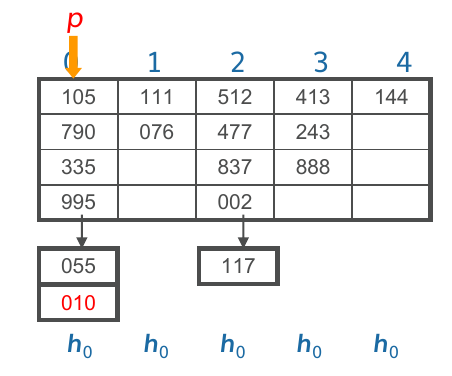
\includegraphics[width=3cm]{images/linearesHashing_1.png}
                \caption{lineares Hashing Schritt 1}
                \label{fig:linHashing1}
            \end{figure}
            
            \begin{figure} [htp]
                \centering
                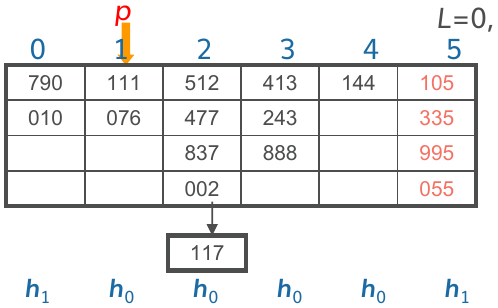
\includegraphics[width=3cm]{images/linearesHashing_2.png}
                \caption{lineares Hashing Schritt 2}
                \label{fig:linHashing2}
            \end{figure}
            
            \item Erweiterbares Hashing
            \begin{itemize}
                \item Buckets werden nur nach Bedarf angelegt
                \item Maximal zwei Seitenzugriffe notwendig
                \item Hashfunktion erzeugt einen Pseudoschlüssel für den Schlüssel
                \item In Buckets werden nur Sätze gespeichert deren Pseudoschlüssel in den ersten d‘ Bit übereinstimmt
                \item d = MAX(d‘) über alle Seiten (globale Tiefe)
                \item Einfügen neuer Schlüssel:
                \begin{enumerate}
                    \item läuft eine Seite über setze d‘ um 1 herauf $\to$ verteile alte Seiteninhalt über zwei Seiten
                    \item falls d dadurch um 1 wächst lege neuen Index mit doppelter Zahl von Einträgen an
                \end{enumerate}
            \end{itemize}
            
            \begin{figure} [htp]
                \centering
                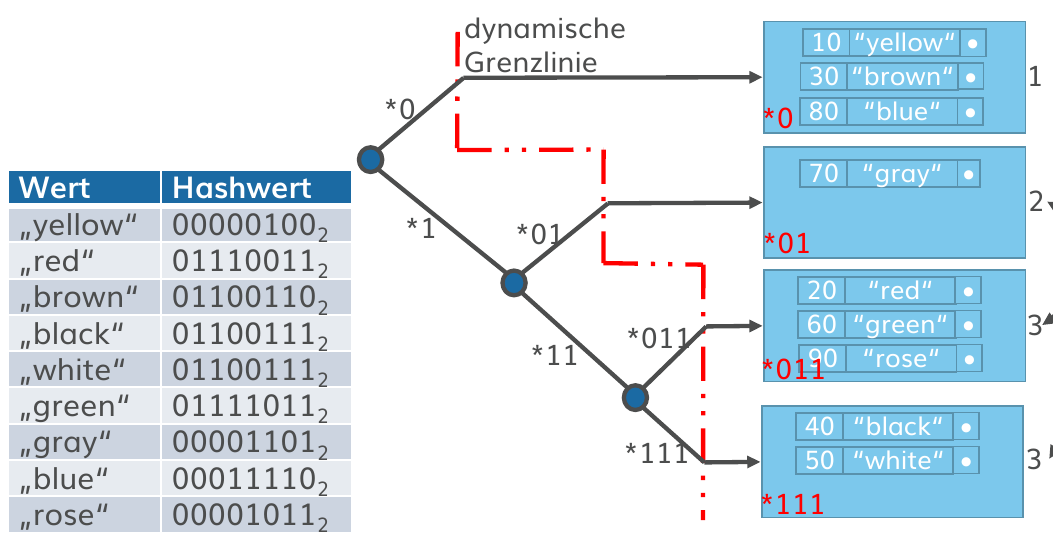
\includegraphics[width=7cm]{images/erweiterbaresHashing.png}
                \caption{erweiterbare Hashing Beispiel}
                \label{fig:erweiterbaresHashing}
            \end{figure}
            
            \item Externes Hashing mit Seperator
            \begin{itemize}
                \item auch bei Überlauf nur 1 Seitenzugriff
                \item Verwendung einer Signaturfunktion zur Zuordnung
                \item Für jeden Bucket gibt es pro Key eine neue Signatur
                \item Ablauf
                \begin{enumerate}
                    \item Bucket Überlauf $\to$ setzen des Bucket Seperator auf die kleinste abgewiesene Signatur 
                    \item abgewiesene Elemente werden in den nächsten Bucket verschoben (siehe Vorgabe)
                \end{enumerate}
                
                \item Einfügen eines Elementes
                \begin{enumerate}
                    \item ist die Signatur größter als der Seperator $\to$ Element kann nicht eingefügt werden $\to$ wahl des nächsten Buckets
                    \item ist die Signatur kleiner als der Seperator $\to$ einfügen
                \end{enumerate}
            \end{itemize}
        \end{itemize}
    \end{enumerate}

\section{Anfrageverarbeitung}



\end{document}
